% 
%	Jan Kechel
%	
%
\documentclass[a4paper,12pt]{report}
\usepackage{epsfig,color,german,graphics}
\pagestyle{headings}
%
\begin{document}
\pagenumbering{roman}
%
\title{MicroOpal\\Programmiersprachen- und systeme\\WS 05/06 TU-Berlin,  Prof. Dr. Peter Pepper}
\author{Jan O. Kechel - Matr.-Nr.: 225136}
\date{01-FEB-2006}
%
\maketitle%
%
\tableofcontents
%
\newpage
\pagenumbering{arabic}
%---------------------------------------------------------------------------
\chapter{Abstrakter Syntaxbaum}
\section{TYPE absy}
Der \texttt{TYPE absy} hat folgende Knoten:
\begin{description}
\item[Prog(ft:absy, rt:absy)] ft = erstes DEF, rt = weiterer Prog-Knoten
\item[Def(funcdecl:absy, funcimpl:absy, toks:seq$\lbrack$token$\rbrack$)] funcdecl = linke seite der Funktion, funcimpl = rechte Seite der Funktion mit Knotentypen ExprTerm, ExprFunc oder ExprCond
\item[FuncDecl(name:string, tp:absy, paramsdecl:absy, toks:seq$\lbrack$token$\rbrack$)] Funktions-Deklaration: name = identifier, type = return-type, paramsdecl sind die Parameter der Funktion
\item[ParamsDecl(ft:absy, rt:absy, toks:seq$\lbrack$token$\rbrack$)] Parameter-Deklaration: ft = erster Parameter, rt = Rest (wieder vom Typ ParamsDecl)
\item[Type(tp:string, toks:seq$\lbrack$token$\rbrack$)] nat oder bool
\item[SingleArg(name:string, tp:absy, toks:seq$\lbrack$token$\rbrack$)] Ein einzelner Parameter in der Funktions-Deklaration mit Name und Typ
\item[ExprTerm(term:string, toks:seq$\lbrack$token$\rbrack$)] Zahl, true oder false
\item[ExprFunc(name:string, params:absy, toks:seq$\lbrack$token$\rbrack$)] Ein Funktions-Aufruf mit Name der Funktion und den Parametern
\item[ExprId(name:string, toks:seq$\lbrack$token$\rbrack$)] eine Variable
\item[Params(ft:absy, rt:absy, toks:seq$\lbrack$token$\rbrack$)] ft = erster Parameter vom Typ Expr*, rt = weitere Parameter (wieder vom Typ Params)
\item[ExprCond(if:absy, then:absy, else:absy, toks:seq$\lbrack$token$\rbrack$)]IF if THEN then ELSE else FI, jeweils vom Type Expr*
\item[Error(error:string, toks:seq$\lbrack$token$\rbrack$)] Fehler-Knoten
\item[Empty(e:string)] Leerer Knoten.
\end{description}
\section{Beispiel}
Die beigelegte fac.mo,
\begin{verbatim}
DEF fac(x:nat):nat ==
    IF eq(x,0) THEN 1 ELSE mul(x, fac(sub(x,1))) FI
DEF MAIN:nat == fac(10)
\end{verbatim}
f"uhrt zu folgendem abstrakten Syntaxbaum (Ausschnitt):
\begin{figure}[h]
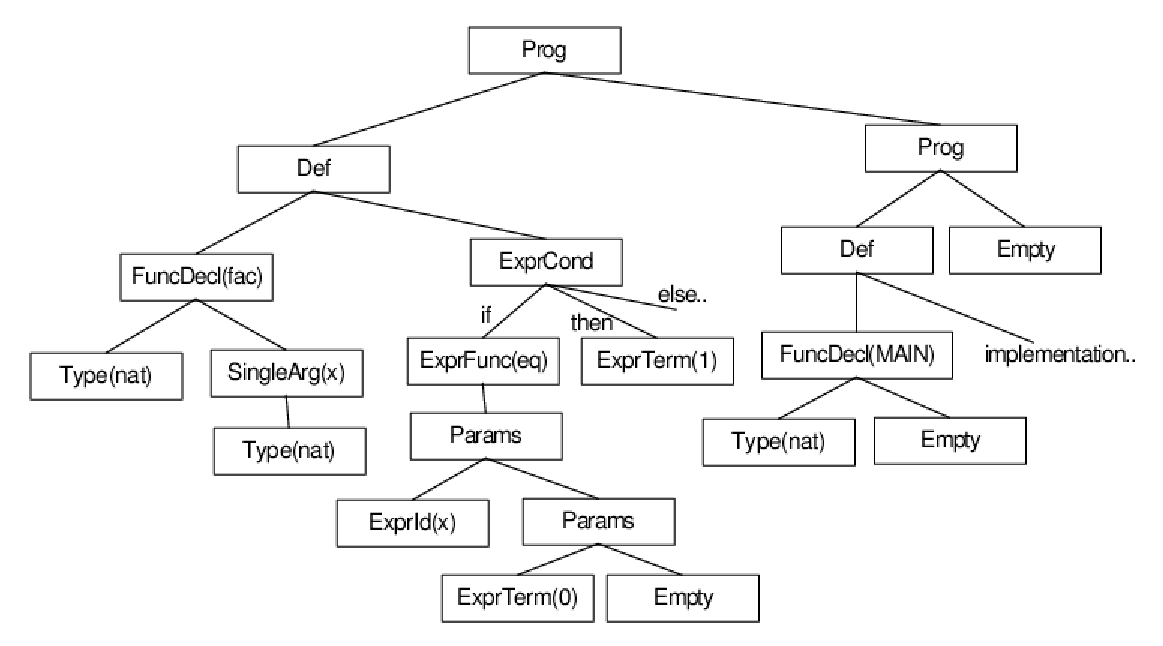
\epsfig{file=absy-fac.eps,width=16cm}
\caption{Beispiel: Absy von fac.mo}
\end{figure}

% ------------------------------------------------------------
% ------------------------------------------------------------
\chapter{Parser}
\section{parsetest}
Dem Parser habe ich eine Funktion \texttt{parsetest} hinzugef"ugt, so da"s er damit aus \texttt{oasys} heraus getestet werden kann:
\begin{verbatim}
>f Parser.impl
Parser.impl>e parsetest("fac")
checking Absy.impl
compiling Absy.impl
starting evaluator process
Prog( Def( FuncDecl: fac( SA(x with Type: nat)SA ) returns (Type: nat), IF
 {   ExprFunc: eq( Params: (id(x), Params: (Term: 0, E)))
 }
 THEN
 {   Term: 1
 }
 ELSE
 {   ExprFunc: mul( Params: (id(x), Params: (
 ExprFunc: fac( Params: (ExprFunc: sub( 
            Params: (id(x), 
            Params: (Term: 1, E))), E)), E)))
 }
 )
 Prog( Def( FuncDecl: MAIN( E) returns (Type: nat), 
            ExprFunc: fac( Params: (Term: 10, E)))
 E))
Parser.impl> 
\end{verbatim}

\section{Tests}
\subsection{Fast alles fehlt noch: tp1.mo}
\begin{verbatim}
DEF MAIN
\end{verbatim}
f"uhrt zu Ergebnis:
\begin{verbatim}
Parser.impl>e parsetest("tp1")
Prog( Def( parseFuncDecl: ':' expected instead of "<EOF>" at global, 
parseFuncImpl: '==' expected  instead of"<EOF>" at global) E)
\end{verbatim}

\subsection{Keine Implementation: tp2.mo}
\begin{verbatim}
DEF MAIN : bool ==
\end{verbatim}
f"uhrt zu Ergebnis:
\begin{verbatim}
Parser.impl>e parsetest("tp2")
Prog( Def( FuncDecl: MAIN( E) returns (Type: bool), 
parseExpression: 'true', 'false', number, function, or IF
expected  instead of "<EOF>" at global) E)
\end{verbatim}

\subsection{Parameterlose Funktion: tp3.mo}
\begin{verbatim}
DEF X : nat == 5
DEF MAIN : bool == false
\end{verbatim}
f"uhrt zu Ergebnis:
\begin{verbatim}
Prog( Def( FuncDecl: X( 
parseParamsDecl: '(' expected instead of ":" at line 1
) returns (Type: nat), Term: 5)
Prog( Def( FuncDecl: MAIN( E) returns (Type: bool), Term: false) E))
\end{verbatim}


\subsection{Viele Fehler gleichzeitig finden: tp4.mo}
\begin{verbatim}
DEF X : nat ==
DEF MAIN : bool == true
DEF Y(b:nat) == 45
DEF Z(b:nat) == IF FI
\end{verbatim}
f"uhrt zu Ergebnis:
\begin{verbatim}
Parser.impl>e parsetest("tp4")
Prog( Def( FuncDecl: X( 
parseParamsDecl: '(' expected instead of ":" at line 1) 
returns (Type: nat), 
parseExpression: 'true', 'false', number, function, or IF expected 
instead of "DEF" at line 2)
Prog( Def( FuncDecl: MAIN( E) returns (Type: bool), Term: true)
Prog( Def( 
parseFuncDecl: ':' expected instead of "==" at line 3, Term: 45)
Prog( Def( 
parseFuncDecl: ':' expected instead of "==" at line 4, 
parseConditional: THEN expected instead of "IF" at line 4) E))))
\end{verbatim}
Hier ist sch"on zu sehen wie das Parsen fortgesetzt wird, obwohl ein Fehler gefunden wurde:
\begin{enumerate}
\item X hat keine Parameter
\item X hat keine Implementation
\item Main wird richtig geparst
\item Y hat keinen return-typ
\item Z hat keinen return-typ
\item Die Implementation von Z hat ein ung"ultiges IF-THEN-ELSE-FI Konstrukt
\end{enumerate}

% ------------------------------------------------------------
% ------------------------------------------------------------
\chapter{Checker}
Wie der Parser hat auch der Syntaxchecker eine Funktion \texttt{checktest} die aus \texttt{oasys} heraus aufgerufen werden kann.

\section{Tests}
\subsection{Keine Main-Funktion: tc1.mo}
\begin{verbatim}
DEF X(a:nat) : bool == false
DEF Y(b:nat) : nat == 5
\end{verbatim}
f"uhrt zu Ergebnis:
\begin{verbatim}
Checker.impl>e checktest("tc1")
checkResult failure: 'ERROR at global: Exactly one MAIN required, found: 0'
\end{verbatim}

\subsection{Zwei Main-Funktionen: tc2.mo}
\begin{verbatim}
DEF MAIN : bool == false
DEF MAIN : nat == 5
\end{verbatim}
f"uhrt zu Ergebnis:
\begin{verbatim}
Checker.impl>e checktest("tc2")
checkResult failure: 'ERROR at line 2: name already exists: MAIN at line 2'
\end{verbatim}

\subsection{Zwei gleichnamige Funktionen: tc3.mo}
\begin{verbatim}
DEF X(a:nat): bool == false
DEF MAIN : nat == 5
DEF X(b:nat): nat == 5
\end{verbatim}
f"uhrt zu Ergebnis:
\begin{verbatim}
Checker.impl>e checktest("tc3")
checkResult failure: 'ERROR at line 3: name already exists: X at line 3'
\end{verbatim}

\subsection{Vordefinierte Funktionsnamen: tc4.mo}
\begin{verbatim}
DEF MAIN : nat == 5
DEF add(a:nat): bool == false
\end{verbatim}
f"uhrt zu Ergebnis:
\begin{verbatim}
Checker.impl>e checktest("tc4")
checkResult failure: 'ERROR at line 2: name already exists: add at line 2
\end{verbatim}

\subsection{Falscher Return-Type: tc5.mo}
\begin{verbatim}
DEF X(a:nat): bool == false
DEF MAIN : nat == X(4)
\end{verbatim}
f"uhrt zu Ergebnis:
\begin{verbatim}
Checker.impl>e checktest("tc5")
checkResult failure: 'ERROR at line 2: Def declaration and implementation 
return different datatypes. DEF declared number but implementation returns 
a boolean"DEF" at line 2'
\end{verbatim}

\subsection{Unterschiedlicher Typ in THEN-ELSE: tc6.mo}
\begin{verbatim}
DEF MAIN : nat == IF true THEN 4 ELSE false FI
\end{verbatim}
f"uhrt zu Ergebnis:
\begin{verbatim}
Checker.impl>e checktest("tc6")
checkResult failure: 'ERROR at line 1: THEN and ELSE part return different 
datatypes THEN: number ELSE: boolean'
\end{verbatim}

\subsection{Falsche Anzahl Parameter: tc7.mo}
\begin{verbatim}
DEF X() : bool == false
DEF MAIN : nat == IF true THEN 4 ELSE X(5) FI
\end{verbatim}
f"uhrt zu Ergebnis:
\begin{verbatim}
Checker.impl>e checktest("tc7")
checkResult failure: 'ERROR at line 2: Too many arguments, 
function 'X' needs less parameters"(" at line 2'
\end{verbatim}

\subsection{Falscher Parameter-Typ: tc8.mo} \begin{verbatim}
DEF X(a:nat) : bool == false
DEF MAIN : nat == IF true THEN 4 ELSE X(false) FI
\end{verbatim}
f"uhrt zu Ergebnis:
\begin{verbatim}
Checker.impl>e checktest("tc7")
checkResult failure: 'ERROR at line 2: Parameter mismatch: 
expected number but got boolean"(" at line 2'
\end{verbatim}

% ------------------------------------------------------------
% ------------------------------------------------------------
\chapter{Interpreter}
Tja, hier gibts nicht viel zu sagen .. er Interpretiert halt. Fehlermeldungen generiere ich hier selber keine, da oasys das ja so sch"on f"ur mich "ubernimmt. Mit der Funktion \texttt{intertest} kann dieser auch aus oasys heraus gestartet werden.

\section{Tests}
\subsection{Negative nat: tc8.mo} \begin{verbatim}
\end{verbatim}
f"uhrt zu Ergebnis:
\begin{verbatim}
Interpreter.impl>e intertest("ti1")
evaluation aborted: `-'Nat: right operand greater than left'
compiled function intertest'Interpreter

jan@janlap:~/uni/pss/microopal$ ./moc ti1.mo
starting execution ...
MAIN == ERROR at global: execution aborted in function MAIN
\end{verbatim}

\section{Benchmark}
Rechner:\\
mobile AMD Athlon(tm) XP2500+\\
cpu MHz         : 1854.633\\
cache size      : 512 KB
\begin{verbatim}
jan@janlap:~/uni/pss/microopal$ time ./moc -i tak.mo
starting interpretation ...
MAIN == 7

real    0m1.012s
user    0m0.966s
sys     0m0.005s
\end{verbatim}


% ------------------------------------------------------------
% ------------------------------------------------------------
\chapter{Compiler}
\section{Tests}
\subsection{fac.mo} 
\begin{verbatim}
jan@janlap:~/uni/pss/microopal$ ./moc fac.mo
starting execution ...
MAIN == 3628800
\end{verbatim}

\subsection{isqrt.mo} 
\begin{verbatim}
jan@janlap:~/uni/pss/microopal$ ./moc isqrt.mo
starting execution ...
MAIN == 3162
\end{verbatim}

\section{Benchmark}
Rechner:\\
mobile AMD Athlon(tm) XP2500+\\
cpu MHz         : 1854.633\\
cache size      : 512 KB
\begin{verbatim}
jan@janlap:~/uni/pss/microopal$ time ./moc tak.mo
starting execution ...
MAIN == 7

real    0m0.774s
user    0m0.728s
sys     0m0.007s
\end{verbatim}



% ------------------------------------------------------------
% ------------------------------------------------------------
\chapter{Bugs}
Mir bekannt Bugs, f"ur die ich aber leider keine Zeit mehr hatte..
\begin{enumerate}
\item Eigene Funktionen ohne Parameter (wie z.B. x():nat) funktionieren nicht
\item Es k"onnen nur Funktionen aufgerufen werden, die vorher definiert wurden
\item Leere Source-Dateien f"uhren zu falscher Fehlermeldung
\item Manche (grammatikalisch falschen) Source-Konstrukte f"uhren zu v"ollig falschen Fehlermeldungen oder Abst"urzen des Parsers
\item 
\end{enumerate}


% ------------------------------------------------------------
% ------------------------------------------------------------
\end{document}
% THE LAST LINE ----------------------------------------------
